\scanpage{215}

$X/S$ lisse, on considère $H^*_{\mathrm{DR}}(X/S)={\unsure{\mathbb H|H}}^*(X,\Omega^*_{X\unsure{/|\,}S})$ et $\mathbb H^*(X,{}^1\Omega_{X/S})$, où ${}^1\Omega_{X/S}=[0\to\underset{\text{degré 1}}{\Omega^1_{X/S}}\to\Omega^{\unsure{2}}_{X/S}\to{-}]$

On a suites spectrales aboutissant à l'une et l'autre, et hom de suites spectrales, donnant un hom de suites exactes en bas degrés

\figure{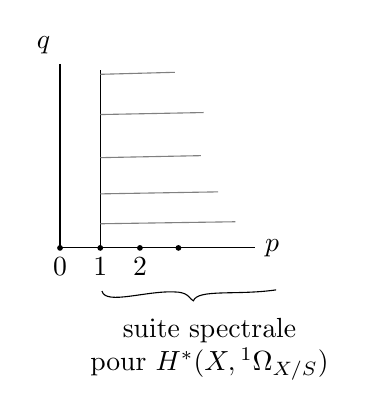
\begin{tikzpicture}[scale=.73]
\draw (0,3.2) node[above left] {$q$} -- (0,0) -- (3.4,0) node[right] {$p$};
\draw (.7,0) -- (.7,3.1);
\foreach \y/\e in {.42/3.05,.94/2.75,1.57/2.45,2.32/2.5,3.02/2.0}{\draw[gray,thin] (.7,\y)--(\e,{\y+.035});}
\foreach \x in {0,.7,1.39,2.06}{\fill (\x,0) circle (.05);}
\node[below] at (0,0){$0$};\node[below] at (.7,0){$1$};\node[below] at (1.39,0){$2$};
\draw (.73,-.75) .. controls (.79,-1.01) and (1.55,-.72) .. (2.06,-.77) .. controls (2.25,-.79) and (2.27,-.91) .. (2.32,-.92) .. controls (2.4,-.71) and (3.07,-.83) .. (3.76,-.73);
\node[below,align=center] at (2.6,-1.05){suite spectrale\\pour $H^*(X,{}^1\Omega_{X/S})$};
\end{tikzpicture}}

\diagram{\resizebox{\linewidth}{!}{\begin{tikzcd}[ampersand replacement=\&,column sep=small,row sep=small]
\&\&{}^{\unsure{1|\prime}}E_2^{10}=Z^1(X,\Omega^*_{X/S})\arrow[ddl]\arrow[d,phantom,"\rotatebox{90}{$\simeq$}" description]
\&\&\&c(\underline L)\arrow[d,phantom,"\rotatebox{-90}{$\in$}" description]
\&\mathrm{Ker}(\mathbb H^1(X,\Omega^1_{X/S})\to H^1(X,\Omega^2_{X/S}))\arrow[d,phantom,"\rotatebox{90}{$\simeq$}" description]\&\\
\&\&H^1(X,{}^1\Omega^*_{X/S})\arrow[d]
\&0\arrow[r]\&{}^1E^{20}_2\arrow[d,phantom,"\rotatebox{90}{$\simeq$}" description]\arrow[r]
\&\mathbb H^2(X,{}^1\Omega^*_{X/S})\arrow[r]\arrow[d]
\&{}^1E_2^{11}\arrow[r]\arrow[d,"\text{surj}"]
\&{}^1E_2^{30}\arrow[d,phantom,"\rotatebox{90}{$\simeq$}" description]\\
0\arrow[r]\&H^1(H^0(X,\Omega^*_{X/S}))\arrow[r]\arrow[d,phantom,"\rotatebox{90}{$=$}" description]
\&H^1_{\mathrm{DR}}(X/S)\arrow[r]
\&\underbrace{\mathrm{Ker}[H^1(X,\underline O_X)\xrightarrow{d}H^1(X,\Omega^1_X)]}_{E^{01}_2}\arrow[r]
\&H^2(H^0(X,\Omega^*))\arrow[r]\arrow[d,phantom,"\rotatebox{90}{$=$}" description]
\&H^2_{\mathrm{DR}}(X)\arrow[r,"\unsure{t}"]
\&H^1(H^1(X,\Omega^*))\arrow[r]\arrow[d,phantom,"\rotatebox{90}{$=$}" description]
\&E_2^{30}\arrow[d,phantom,"\rotatebox{90}{$=$}" description]\\
\&E^{10}_2=\dfrac{Z^1(X,\Omega^*_{X/S})}{\mathrm{Im}\,C^0(X,\Omega^*_{X/S})}
\&\&\&E^{20}_2=\dfrac{Z^2(X,\Omega^*_{X/S})}{\mathrm{Im}\,C^{\unsure{1|0}}(X,\Omega^*_{X/S})}
\&\&E^{11}_2=\dfrac{\mathrm{Ker}[H^1(X,\Omega^1)\to H^1(X,\Omega^2)]}{\mathrm{Im}[H^1(X,\Omega^0)\to H^1(X,\Omega^1]}\&\cdots
\end{tikzcd}}}

Pour que $\exists$ connexion intégrable sur $\underline L$, module inv. donné sur $X$, il faut que l'obstruction en $\mathbb H^2(X,{}^1\Omega^*_{X/S})$ soit nulle, i.e

\textcircled{a} \deleted{$\unsure{H}$} $c^1_{\mathrm{Hdg}}(L)\in H^1(X,\Omega^1_{X/S})$ nul

\textcircled{b} deuxième obstruction dans $H^2(H^0(X,\Omega^*))=\dfrac{Z^2(X,\Omega^*_{X/S})}{\mathrm{Im}\,\unsure{C^1|d}(X,\Omega^{\unsure{0|*}}_{X/S})}$ soit nulle.

\uline{NB} En car. $p>0$, l'obstruction est ds un $\unsure{\mathbb F_p|F_p}$-vectoriel, donc tué par $p$. Donc \inserted{pour} tout élt de $p\,\mathrm{Pic}(X)$ l'obstruction est nulle. On présume, si $X$ est propre sur $S$, \inserted{loclt}, que l'obstruction est nulle \deleted{dans} si $\xi$ est ds $\mathrm{Pic}^0(X/S)$ (à vérifier \ldots).

Supposons l'obstruction en question nulle, \inserted{$S$ de car $p>0$,} Alors l'indétermination pour trouver la connexion intégrable est un $Z^1(X,\Omega^*_{X/S})$, i.e. c'est une 1-forme relative $\omega$ \uline{fermée} ($d\omega=0$). \deleted{A quelle} \deleted{Donc $C$} D'autre part, le \uline{défaut} \uline{de compatibilité} \uline{aux puiss. $p^{\mathrm{ièmes}}$} est un \deleted{homomorphisme} à hom additif et $p$-homogène ${\unsure{\mathscr T|\mathscr U|\underline V}}_{X/S}\longrightarrow\underline{\mathrm{End}}(\underline L)\deleted{\unsure{\simeq}}$, i.e. un hom $u:\mathscr T^{(p)}_{X/S}\longrightarrow\mathrm{End}(\underline L)$, i.e. ici une section de $\underline\Omega^1_{X/S}{}^{(p)}$. Cette section, si on remplace la connexion $\Theta^{{}}$ par $\Theta'=\Theta+\omega$, est remplacée par

% slanted
\margin{résulte des formules explicites}

\[
\begin{aligned}
&\deleted{\xi\longmapsto}u'(\xi)=u(\xi)+\underbrace{\omega(\xi)^p\deleted{\unsure{\omega(\xi)}}+\Theta_\xi^{p-1}\omega(\xi)-\omega(\xi^p)}
=u(\xi)+\underbrace{\omega(\xi)^p-\deleted{\unsure{C_\xi}}\langle\underset{\text{opération de Cartier}}{C}\omega,\widetilde\xi\rangle1_{\unsure{\underline\Lambda|\underline L}}}\\
&=
\end{aligned}
\]

% archive sheet number: 214
